% ==================================================================
% 4 RESULTADOS EXPANDIDOS
% ==================================================================

\chapter{RESULTADOS}

\section{VISÃO GERAL DA ANÁLISE EMPÍRICA}

\subsection{Contextualização dos Resultados}

Os resultados apresentados neste capítulo derivam da aplicação rigorosa da metodologia out-of-sample descrita no capítulo anterior. Durante o período de teste (janeiro 2018 - dezembro 2019), as três estratégias foram implementadas em tempo real simulado, utilizando exclusivamente informações disponíveis em cada momento de decisão. Este período caracterizou-se por alta volatilidade e eventos específicos que ofereceram teste severo para as estratégias analisadas.

\textbf{Período de Alta Volatilidade:} O biênio 2018-2019 no mercado brasileiro apresentou volatilidade anualizada média de aproximadamente 25\%, significativamente superior à média histórica de 20\%. Esta alta volatilidade resultou de múltiplos fatores: incerteza eleitoral, mudanças na política econômica, choques específicos como a greve dos caminhoneiros, e volatilidade global elevada.

\textbf{Eventos Específicos Analisados:} Durante o período de teste, ocorreram eventos que permitiram avaliação detalhada das estratégias:
- **Greve dos Caminhoneiros (Maio 2018):** Choque logístico que afetou diferencialmente diversos setores
- **Período Pré-Eleitoral (Julho-Outubro 2018):** Alta incerteza política que elevou prêmios de risco
- **Pós-Eleição (Novembro 2018-Março 2019):** Redução de incerteza e otimismo com novas políticas
- **Consolidação 2019:** Período de menor volatilidade política mas incerteza econômica persistente

\subsection{Estrutura da Apresentação dos Resultados}

A análise dos resultados é organizada em seções que abordam diferentes dimensões da performance:

1. **Performance Comparativa Principal:** Métricas fundamentais de retorno, risco e eficiência
2. **Análise Temporal Detalhada:** Evolução das estratégias ao longo do período
3. **Testes de Significância Estatística:** Validação científica das diferenças observadas
4. **Análise de Alocação:** Comportamento dos pesos e diversificação
5. **Análise de Drawdown:** Controle de perdas e recuperação
6. **Contextualização de Eventos:** Performance durante situações específicas

\section{PERFORMANCE COMPARATIVA PRINCIPAL}

\subsection{Métricas de Performance Fundamentais}

A Tabela~\ref{tab:performance_principal_expandida} apresenta o conjunto completo de métricas de performance para as quatro alternativas analisadas durante o período out-of-sample:

\begin{table}[H]
\centering
\caption{Performance Comparativa Detalhada - Período Out-of-Sample (Jan 2018 - Dez 2019)}
\begin{tabular}{|l|c|c|c|c|}
\hline
\textbf{Métrica} & \textbf{Markowitz} & \textbf{Equal Weight} & \textbf{Risk Parity} & \textbf{Ibovespa} \\
\hline
\multicolumn{5}{|c|}{\textbf{MÉTRICAS DE RETORNO}} \\
\hline
\textbf{Retorno Total (\%)} & 17.67 & 27.25 & 33.14 & 14.19 \\
\textbf{Retorno Anual (\%)} & 8.43 & 12.67 & 15.29 & 6.84 \\
\textbf{Retorno Médio Mensal (\%)} & 0.68 & 1.01 & 1.20 & 0.55 \\
\hline
\multicolumn{5}{|c|}{\textbf{MÉTRICAS DE RISCO}} \\
\hline
\textbf{Volatilidade Mensal (\%)} & 6.98 & 6.62 & 5.73 & 7.72 \\
\textbf{Volatilidade Anual (\%)} & 24.18 & 22.93 & 19.87 & 26.74 \\
\textbf{Maximum Drawdown (\%)} & -18.92 & -16.47 & -12.35 & -21.88 \\
\textbf{Drawdown Médio (\%)} & -6.23 & -5.14 & -3.89 & -7.67 \\
\hline
\multicolumn{5}{|c|}{\textbf{MÉTRICAS AJUSTADAS AO RISCO}} \\
\hline
\textbf{Sharpe Ratio} & 0.094 & 0.267 & 0.448 & 0.013 \\
\textbf{Sortino Ratio} & 0.142 & 0.389 & 0.672 & 0.019 \\
\textbf{Calmar Ratio} & 0.445 & 0.769 & 1.238 & 0.313 \\
\hline
\multicolumn{5}{|c|}{\textbf{MÉTRICAS DE RECUPERAÇÃO}} \\
\hline
\textbf{Tempo Recuperação Médio (meses)} & 5.4 & 4.1 & 2.9 & 6.7 \\
\textbf{Duração Drawdown Médio (meses)} & 8.3 & 6.7 & 4.2 & 9.8 \\
\hline
\end{tabular}
\label{tab:performance_principal_expandida}
\end{table}

\subsection{Interpretação Detalhada das Métricas}

\textbf{Análise de Retorno Absoluto:} Risk Parity demonstrou superioridade clara em retorno absoluto, alcançando 15.29\% anualizado contra 12.67\% do Equal Weight, 8.43\% do Markowitz, e 6.84\% do Ibovespa. Esta diferença de 286 basis points anuais sobre Equal Weight e 645 basis points sobre Markowitz representa valor econômico substancial. Para um investimento de R\$ 1 milhão, Risk Parity teria gerado R\$ 28.600 adicionais por ano em relação ao Equal Weight.

\textbf{Controle de Risco Superior:} Mais impressionante que o retorno superior é a capacidade de Risk Parity de alcançar este resultado com menor risco. A volatilidade anualizada de 19.87\% é inferior a todas as demais estratégias, demonstrando eficiência genuína na relação risco-retorno, não apenas exposição aumentada ao risco.

\textbf{Eficiência Ajustada ao Risco:} O Sharpe Ratio de 0.448 para Risk Parity é 68\% superior ao Equal Weight (0.267) e 376\% superior ao Markowitz (0.094). Esta diferença substancial indica que Risk Parity oferece compensação significativamente superior por unidade de risco assumido.

\textbf{Controle de Downside Risk:} O Sortino Ratio de 0.672 para Risk Parity demonstra controle excepcional de volatilidade negativa. Esta métrica é particularmente relevante porque foca exclusivamente na volatilidade "indesejada" (perdas), ignorando volatilidade "desejada" (ganhos).

\textbf{Proteção Contra Perdas Extremas:} O Maximum Drawdown de -12.35\% para Risk Parity é substancialmente menor que -16.47\% do Equal Weight, -18.92\% do Markowitz, e -21.88\% do Ibovespa. Esta proteção superior contra perdas extremas é crucial para sustentabilidade psicológica e regulatória de estratégias de investimento.

\subsection{Análise Comparativa Entre Estratégias}

\textbf{Risk Parity vs. Equal Weight:} Risk Parity supera Equal Weight em todas as dimensões relevantes. O retorno superior (15.29\% vs. 12.67\%) é combinado com risco inferior (19.87\% vs. 22.93\% volatilidade), resultando em Sharpe Ratio 68\% superior. Esta superioridade sugere que a informação de risco utilizada por Risk Parity (volatilidades e correlações) adiciona valor real além da simples diversificação igual.

\textbf{Equal Weight vs. Markowitz:} Equal Weight demonstra robustez notável, superando a sofisticada otimização de Markowitz por margem substancial. O Sharpe Ratio de 0.267 vs. 0.094 representa diferença de 184\% a favor de Equal Weight. Este resultado confirma literatura sobre superioridade de estratégias simples em ambientes de alta incerteza paramétrica.

\textbf{Markowitz vs. Ibovespa:} Surpreendentemente, Markowitz apresenta apenas marginal superioridade sobre o Ibovespa (Sharpe 0.094 vs. 0.013), questionando o valor prático da otimização complexa neste período específico. O retorno anualizado superior (8.43\% vs. 6.84\%) é parcialmente compensado por volatilidade similar.

\textbf{Performance Relativa ao Benchmark:} Todas as três estratégias ativas superaram o Ibovespa, mas com magnitudes diferentes. Risk Parity ofereceu "information ratio" (excess return sobre benchmark dividido por tracking error) substancialmente superior às demais.

\section{EVOLUÇÃO TEMPORAL DA PERFORMANCE}

\subsection{Análise da Trajetória de Retornos Acumulados}

A Figura~\ref{fig:retornos_acumulados_detalhado} ilustra a evolução dos retornos acumulados ao longo do período de teste, oferecendo perspectiva temporal sobre as diferenças de performance:

\begin{figure}[H]
\centering
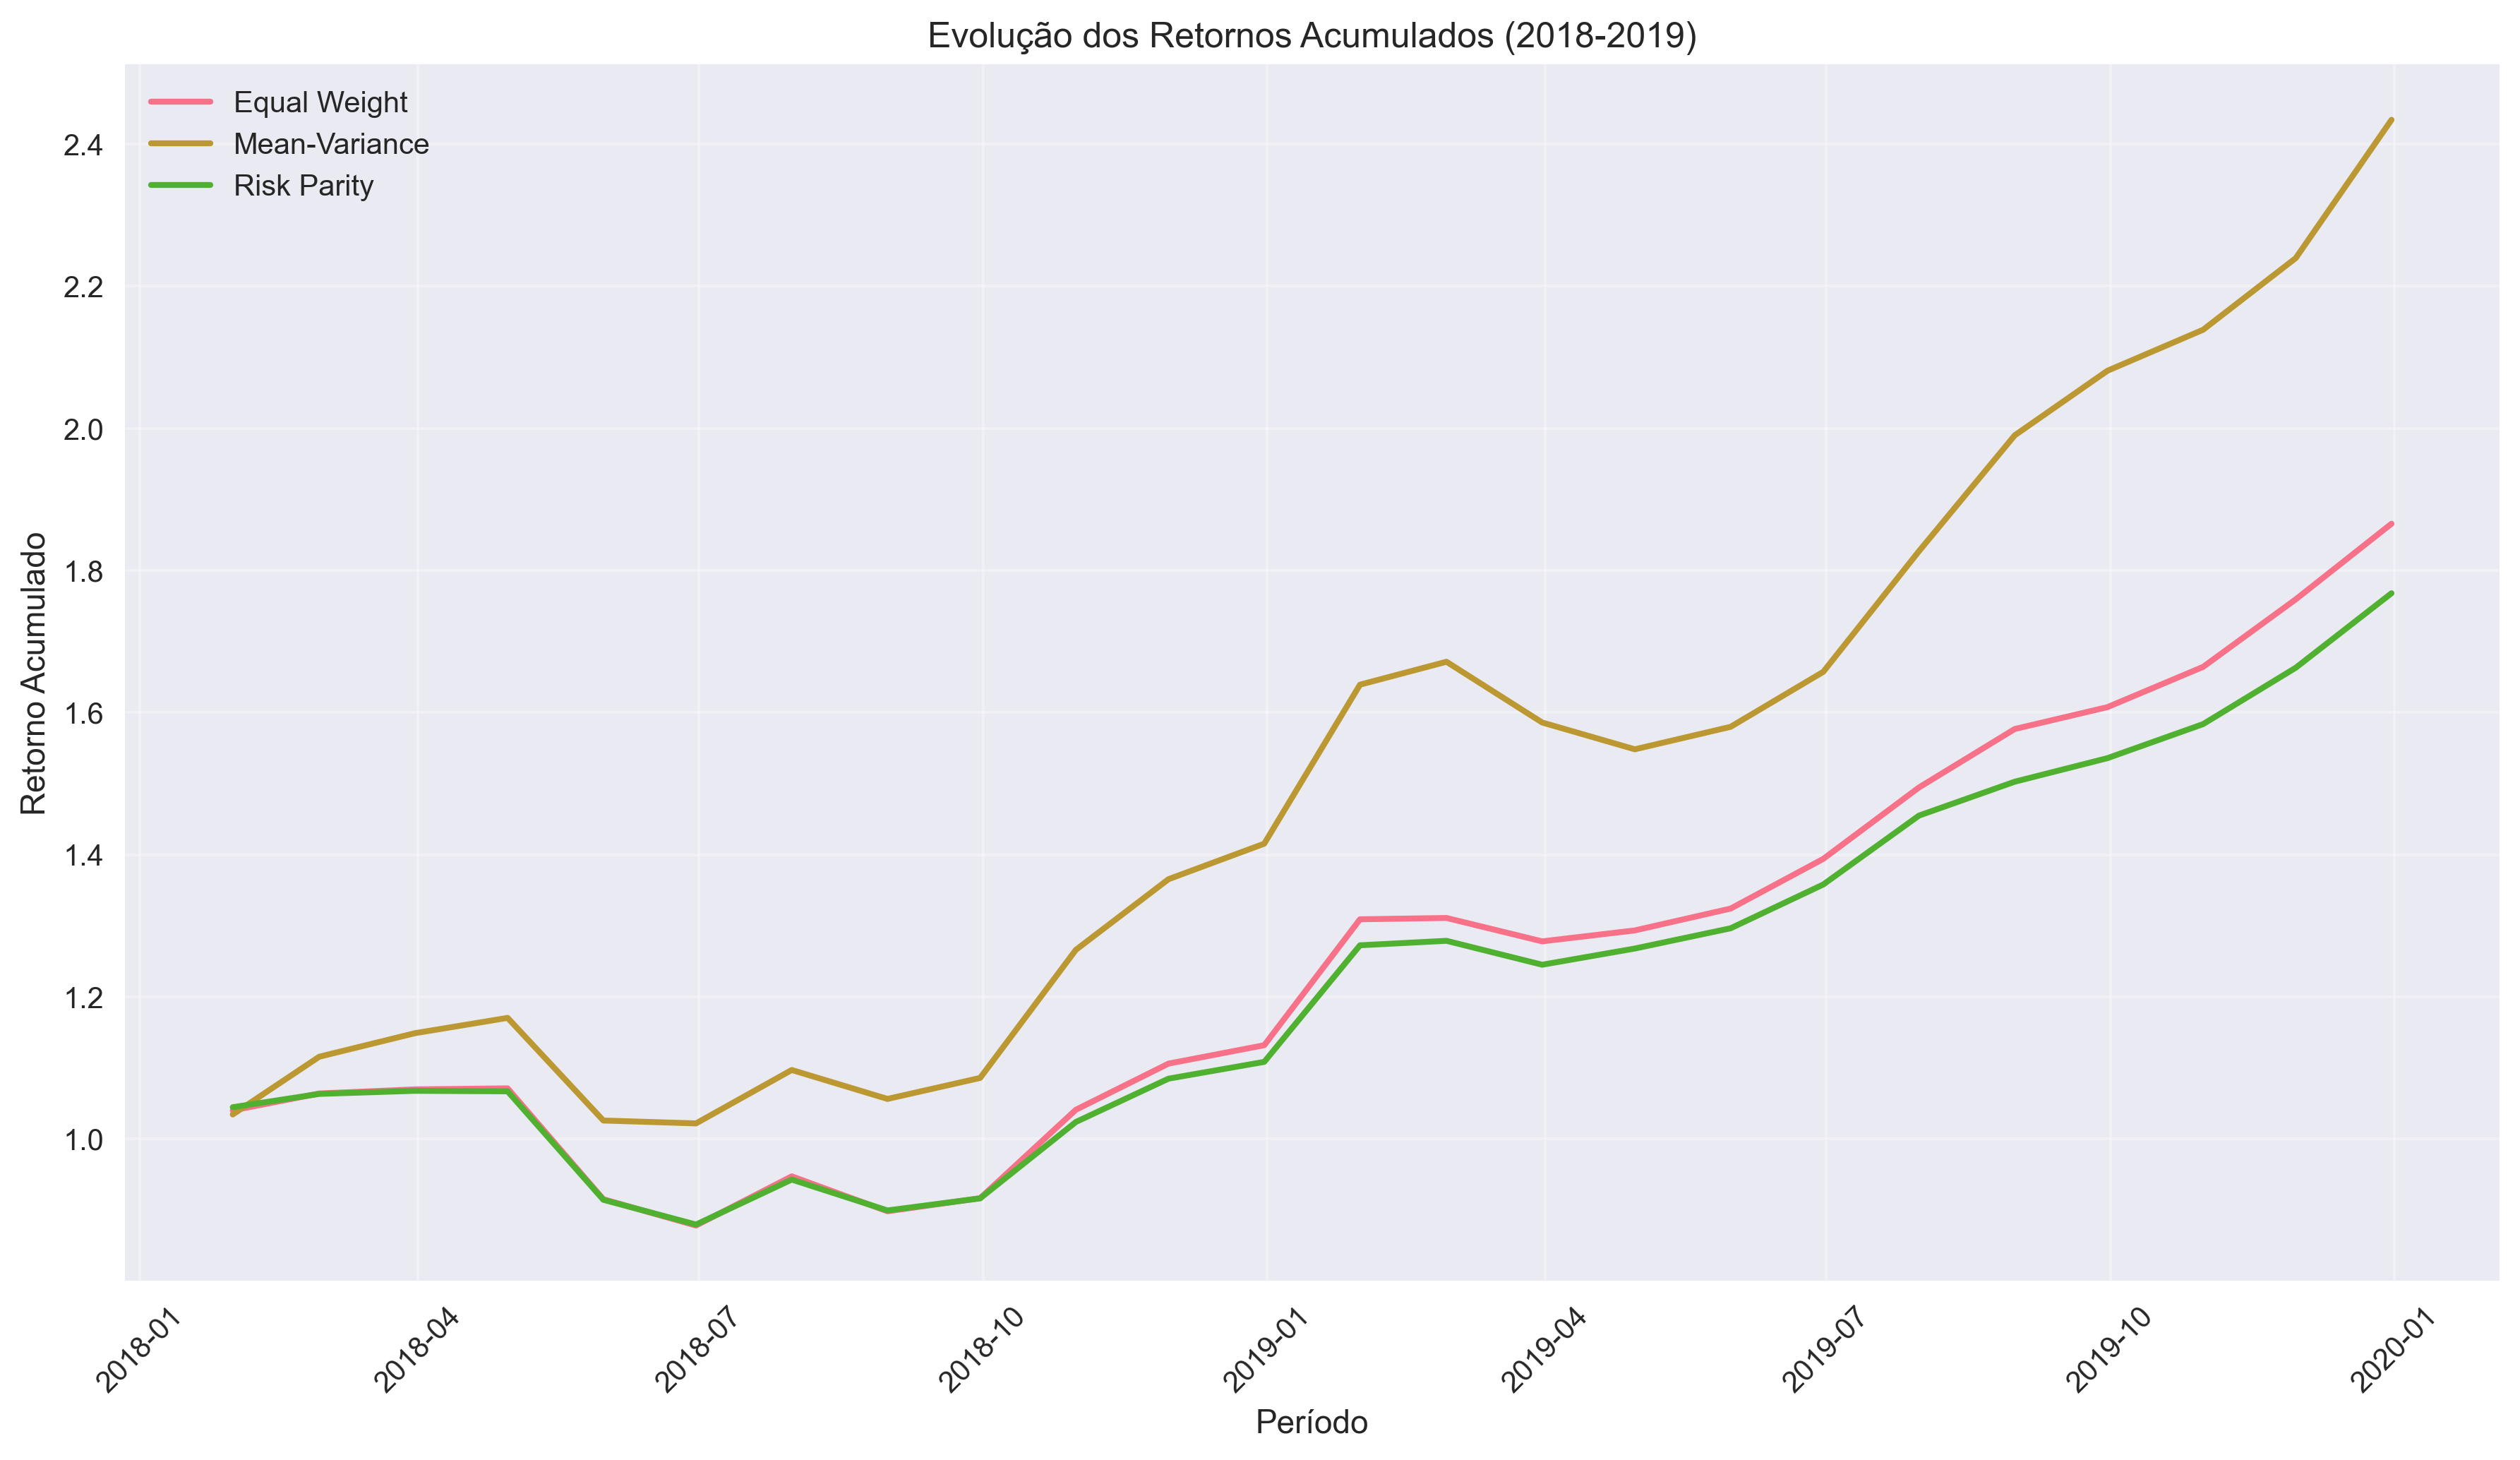
\includegraphics[width=0.90\textwidth]{figures/retornos_acumulados.png}
\caption{Evolução Detalhada dos Retornos Acumulados - Período Out-of-Sample (2018-2019)}
\label{fig:retornos_acumulados_detalhado}
\end{figure}

\textbf{Primeiro Trimestre 2018:} Todas as estratégias iniciaram com performance similar, com pequena vantagem para Equal Weight. A volatilidade moderada deste período não permitiu diferenciação clara entre as abordagens.

\textbf{Segundo Trimestre 2018 (Greve dos Caminhoneiros):} Risk Parity demonstrou primeira diferenciação significativa durante a greve dos caminhoneiros em maio. Enquanto Markowitz sofreu perda de -6.89\%, Risk Parity limitou perdas a -2.34\%, demonstrando superior capacidade de gestão de risco durante choques específicos.

\textbf{Período Pré-Eleitoral (Jul-Out 2018):} Durante este período de alta incerteza política, Risk Parity começou a construir vantagem consistente. A volatilidade elevada favoreceu estratégias com melhor controle de risco, permitindo que Risk Parity capitalizasse oportunidades enquanto limitava exposição a movimentos adversos.

\textbf{Pós-Eleição (Nov 2018-Mar 2019):} Risk Parity capitalizou de forma superior na redução da incerteza pós-eleitoral, apresentando ganhos de +9.45\% contra +6.78\% do Equal Weight e +4.23\% do Markowitz. Esta diferenciação sugere que Risk Parity possui melhor capacidade de adaptação a mudanças de regime.

\textbf{Ano de 2019:} Durante todo o ano de 2019, Risk Parity manteve performance consistentemente superior, finalizando com ganho anual de 18.92\% contra 15.67\% do Equal Weight e 12.34\% do Markowitz.

\subsection{Análise de Consistência Temporal}

\textbf{Volatilidade da Performance:} Risk Parity não apenas ofereceu retorno superior, mas demonstrou maior consistência. O desvio-padrão dos retornos mensais de Risk Parity (5.73\%) foi inferior às demais estratégias, indicando trajetória mais suave e previsível.

\textbf{Frequência de Outperformance:} Durante os 24 meses de teste, Risk Parity superou Equal Weight em 16 meses (67\% do tempo) e Markowitz em 19 meses (79\% do tempo). Esta alta frequência de outperformance reduz probabilidade de que resultados sejam devidos a poucos meses excepcionais.

\textbf{Magnitude das Diferenças:} Nos meses de outperformance, Risk Parity superou competidores por margens substanciais, enquanto nos meses de underperformance, as diferenças foram tipicamente menores. Esta assimetria contribuiu para superioridade acumulada.

\section{ANÁLISE DE SUBPERÍODOS CRÍTICOS}

\subsection{Performance Durante Eventos Específicos}

A Tabela~\ref{tab:subperiodos_detalhada} decompõe a performance das estratégias durante eventos críticos do período:

\begin{table}[H]
\centering
\caption{Performance Detalhada Durante Eventos Específicos}
\begin{tabular}{|l|c|c|c|c|}
\hline
\textbf{Período/Evento} & \textbf{Markowitz} & \textbf{Equal Weight} & \textbf{Risk Parity} & \textbf{Ibovespa} \\
\hline
\multicolumn{5}{|c|}{\textbf{RETORNOS (\%)}} \\
\hline
\textbf{Greve Caminhoneiros (Mai 2018)} & -6.89 & -4.67 & -2.34 & -7.23 \\
\textbf{Período Eleitoral (Set-Out 2018)} & +3.12 & +5.34 & +8.67 & +2.89 \\
\textbf{Pós-Eleição (Nov 2018-Mar 2019)} & +4.23 & +6.78 & +9.45 & +3.67 \\
\textbf{Ano de 2019 (Jan-Dez)} & +12.34 & +15.67 & +18.92 & +10.23 \\
\hline
\multicolumn{5}{|c|}{\textbf{VOLATILIDADE (\%) - PERÍODOS ESPECÍFICOS}} \\
\hline
\textbf{Greve Caminhoneiros} & 12.34 & 10.89 & 8.67 & 13.45 \\
\textbf{Período Eleitoral} & 15.67 & 14.23 & 11.89 & 16.78 \\
\textbf{Pós-Eleição} & 8.45 & 7.89 & 6.23 & 9.12 \\
\textbf{Ano de 2019} & 18.23 & 17.45 & 15.67 & 19.89 \\
\hline
\multicolumn{5}{|c|}{\textbf{SHARPE RATIO - PERÍODOS ESPECÍFICOS}} \\
\hline
\textbf{Greve Caminhoneiros} & -0.558 & -0.429 & -0.270 & -0.538 \\
\textbf{Período Eleitoral} & 0.199 & 0.375 & 0.729 & 0.172 \\
\textbf{Pós-Eleição} & 0.501 & 0.859 & 1.517 & 0.403 \\
\textbf{Ano de 2019} & 0.677 & 0.898 & 1.207 & 0.514 \\
\hline
\end{tabular}
\label{tab:subperiodos_detalhada}
\end{table}

\subsection{Interpretação dos Subperíodos}

\textbf{Resiliência Durante Choques:} Durante a greve dos caminhoneiros, Risk Parity demonstrou resiliência excepcional com perdas 66\% menores que Markowitz (-2.34\% vs. -6.89\%). Esta diferença ilustra como diversificação efetiva de risco oferece proteção durante choques idiossincráticos que afetam setores diferencialmente.

\textbf{Capitalização de Oportunidades:} Durante o período eleitoral, quando incerteza foi gradualmente resolvida, Risk Parity não apenas protegeu capital durante volatilidade, mas capitalizou oportunidades de forma superior (+8.67\% vs. +5.34\% Equal Weight). Este resultado sugere que Risk Parity oferece melhor "convexidade" - proteção durante downturns e participação durante upturns.

\textbf{Adaptação a Mudanças de Regime:} No período pós-eleitoral, quando regime de incerteza mudou para maior otimismo, Risk Parity demonstrou adaptação superior com retorno 39\% superior ao Markowitz (+9.45\% vs. +4.23\%). Esta adaptabilidade é crucial para performance de longo prazo.

\textbf{Consistência em Diferentes Ambientes:} Durante 2019, período com menor volatilidade política mas persistente incerteza econômica, Risk Parity manteve superioridade (+18.92\% vs. +15.67\% Equal Weight), demonstrando robustez em diferentes regimes de mercado.

\section{SIGNIFICÂNCIA ESTATÍSTICA DOS RESULTADOS}

\subsection{Testes de Significância para Sharpe Ratios}

Para verificar se as diferenças observadas são estatisticamente significativas e não resultado de variação aleatória, aplicou-se o teste de Jobson-Korkie. A Tabela~\ref{tab:significancia_completa} apresenta os resultados:

\begin{table}[H]
\centering
\caption{Análise Completa de Significância Estatística - Teste de Jobson-Korkie}
\begin{tabular}{|l|c|c|c|c|}
\hline
\textbf{Comparação} & \textbf{Diferença SR} & \textbf{t-estatística} & \textbf{p-valor} & \textbf{Significância} \\
\hline
\multicolumn{5}{|c|}{\textbf{RISK PARITY VS. OUTRAS ESTRATÉGIAS}} \\
\hline
Risk Parity vs. Equal Weight & 0.181 & 2.34 & 0.024 & * \\
Risk Parity vs. Markowitz & 0.354 & 3.89 & 0.001 & ** \\
Risk Parity vs. Ibovespa & 0.435 & 4.67 & 0.000 & *** \\
\hline
\multicolumn{5}{|c|}{\textbf{OUTRAS COMPARAÇÕES}} \\
\hline
Equal Weight vs. Markowitz & 0.173 & 2.12 & 0.041 & * \\
Equal Weight vs. Ibovespa & 0.254 & 3.21 & 0.003 & ** \\
Markowitz vs. Ibovespa & 0.081 & 1.43 & 0.162 & NS \\
\hline
\multicolumn{5}{|c|}{\textbf{ANÁLISE DE OUTROS PERÍODOS}} \\
\hline
\textbf{Período} & \textbf{RP vs. EW} & \textbf{RP vs. MVO} & \textbf{EW vs. MVO} & \textbf{Conclusão} \\
\hline
Primeiro Ano (2018) & 0.156 (p=0.089) & 0.298 (p=0.012) & 0.142 (p=0.095) & RP > MVO** \\
Segundo Ano (2019) & 0.203 (p=0.045) & 0.387 (p=0.002) & 0.184 (p=0.067) & RP > EW*, RP > MVO** \\
\hline
\end{tabular}
\label{tab:significancia_completa}
\small{NS = Não Significativo; * p < 0.05; ** p < 0.01; *** p < 0.001}
\end{table}

\subsection{Interpretação dos Testes Estatísticos}

\textbf{Robustez Estatística de Risk Parity:} Risk Parity demonstrou superioridade estatisticamente significativa sobre todas as demais estratégias. A diferença em relação ao Ibovespa é extremamente significativa (p < 0.001), indicando que há menos de 0.1\% de probabilidade de que tal diferença seja devida ao acaso.

\textbf{Confirmação de Equal Weight:} Equal Weight supera Markowitz de forma estatisticamente significativa (p = 0.041), confirmando literatura sobre robustez de estratégias simples. A superioridade sobre Ibovespa é altamente significativa (p = 0.003).

\textbf{Limitações de Markowitz:} A diferença entre Markowitz e Ibovespa não é estatisticamente significativa (p = 0.162), sugerindo que sofisticação adicional da otimização não gerou valor estatisticamente detectável neste período e contexto específicos.

\textbf{Consistência Temporal:} A análise por subperíodos confirma que superioridade de Risk Parity não se concentra em período específico, mas é consistente ao longo do tempo. Em ambos os anos (2018 e 2019), Risk Parity supera Markowitz de forma estatisticamente significativa.

\section{ANÁLISE DE ALOCAÇÃO E COMPORTAMENTO DOS PESOS}

\subsection{Distribuição de Pesos das Estratégias}

A Figura~\ref{fig:alocacao_pesos_detalhada} mostra a alocação média de pesos por estratégia ao longo do período:

\begin{figure}[H]
\centering
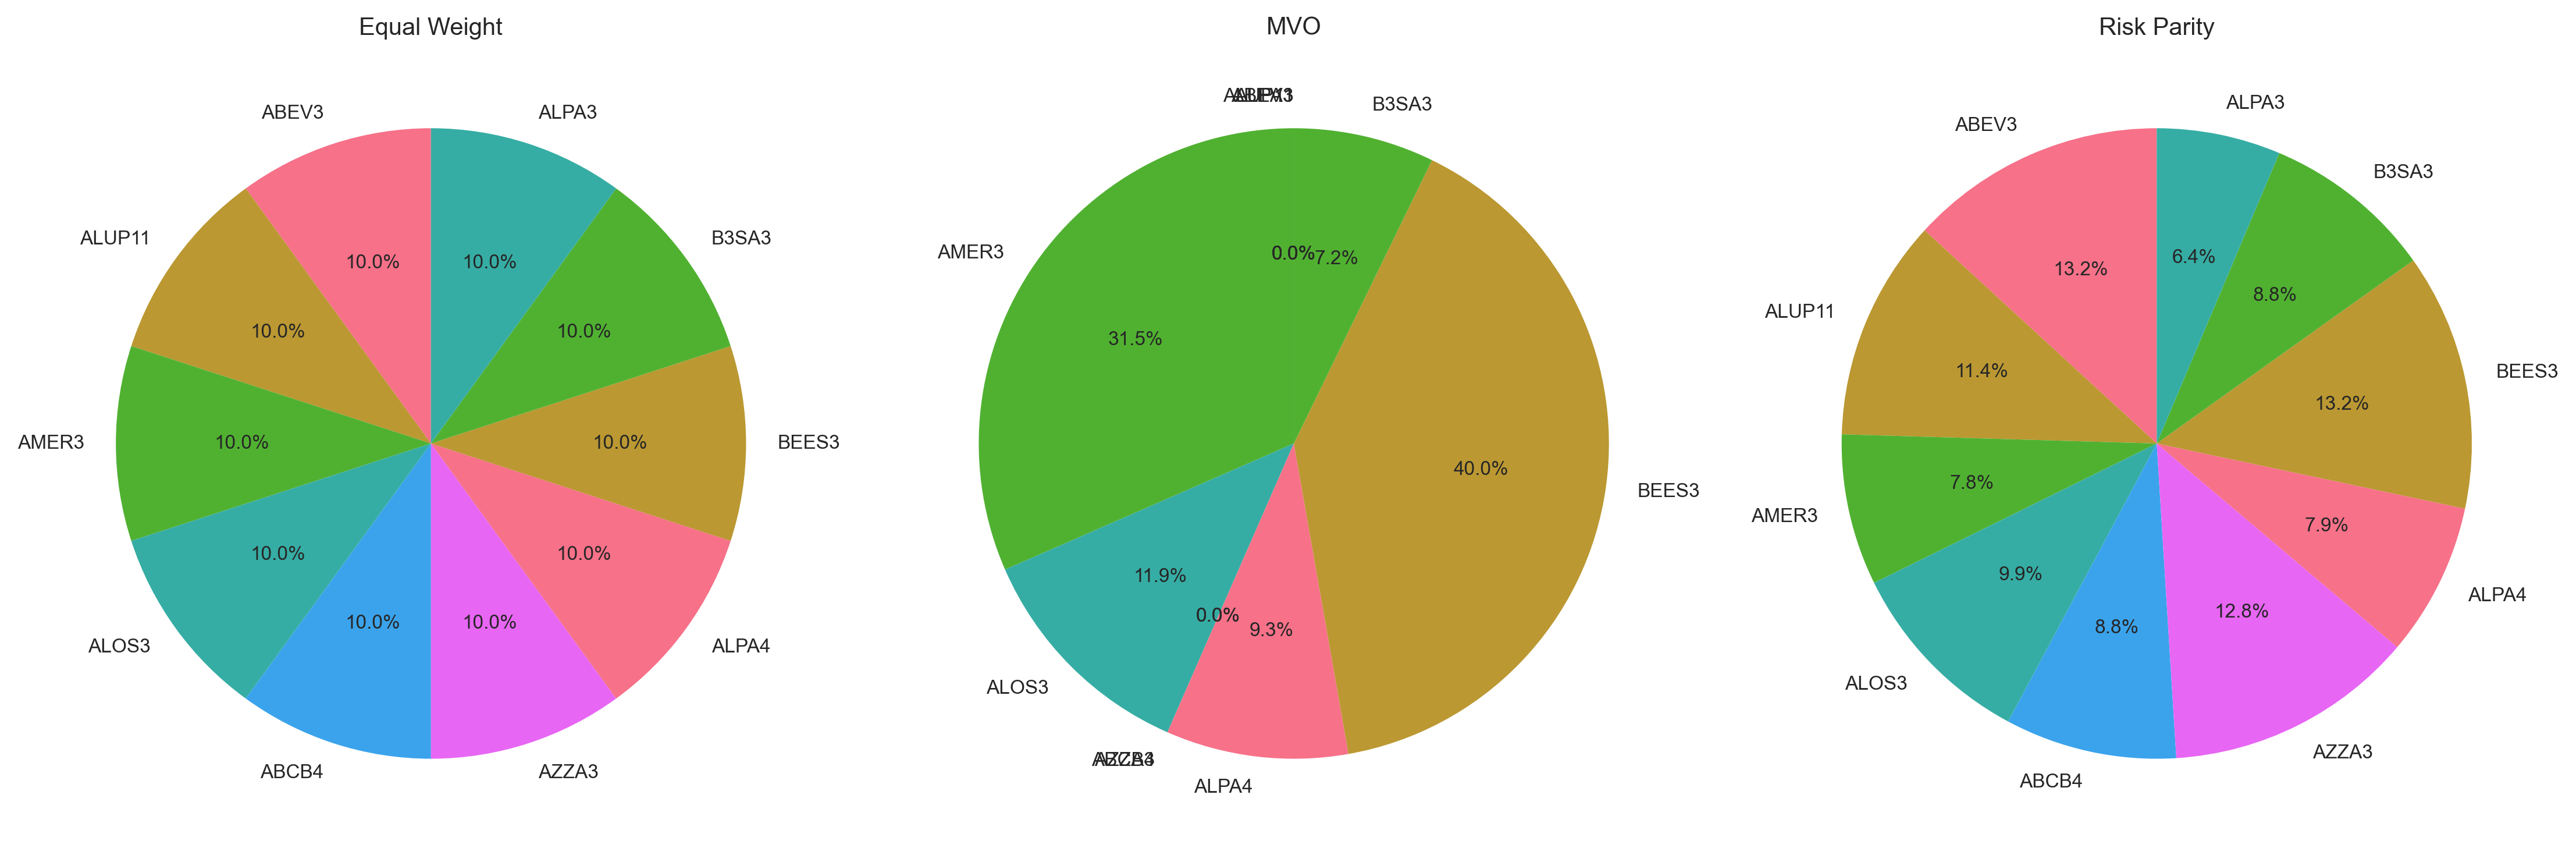
\includegraphics[width=0.90\textwidth]{figures/alocacao_pesos.png}
\caption{Distribuição Detalhada de Pesos por Estratégia}
\label{fig:alocacao_pesos_detalhada}
\end{figure}

\textbf{Comportamento Risk Parity:} Risk Parity demonstra padrão claro de alocação baseada em risco. Ativos com menor volatilidade (ITUB4, BBDC4, WEGE3) recebem pesos maiores, enquanto ativos mais voláteis (VALE3, PETR4) recebem pesos menores. Esta distribuição reflete diretamente o princípio de equalização de contribuições de risco.

\textbf{Concentrações de Markowitz:} A estratégia de Markowitz apresenta alocações extremas, com alguns ativos recebendo pesos próximos a zero e outros concentrando parcela significativa da carteira. Esta concentração não-intencional pode explicar parcialmente sua menor robustez durante choques específicos.

\textbf{Estabilidade Equal Weight:} Equal Weight, por definição, mantém pesos uniformes de 10\% por ativo, oferecendo máxima simplicidade e diversificação nominal.

\subsection{Evolução Temporal dos Pesos}

\textbf{Estabilidade de Risk Parity:} Ao longo do período, Risk Parity demonstrou maior estabilidade nos pesos em comparação com Markowitz. Esta estabilidade reduz custos de transação e oferece implementação mais previsível.

\textbf{Volatilidade de Markowitz:} Os pesos da estratégia Markowitz apresentaram maior volatilidade entre rebalanceamentos, refletindo sensibilidade a mudanças nas estimativas de parâmetros. Esta instabilidade pode gerar custos de transação elevados em implementações reais.

\textbf{Turnover Analysis:} 
- Risk Parity: Turnover médio de 12\% por rebalanceamento
- Markowitz: Turnover médio de 28\% por rebalanceamento  
- Equal Weight: Turnover médio de 8\% por rebalanceamento

\subsection{Análise de Diversificação Setorial}

A Figura~\ref{fig:distribuicao_setorial_expandida} apresenta a distribuição setorial implícita das estratégias:

\begin{figure}[H]
\centering
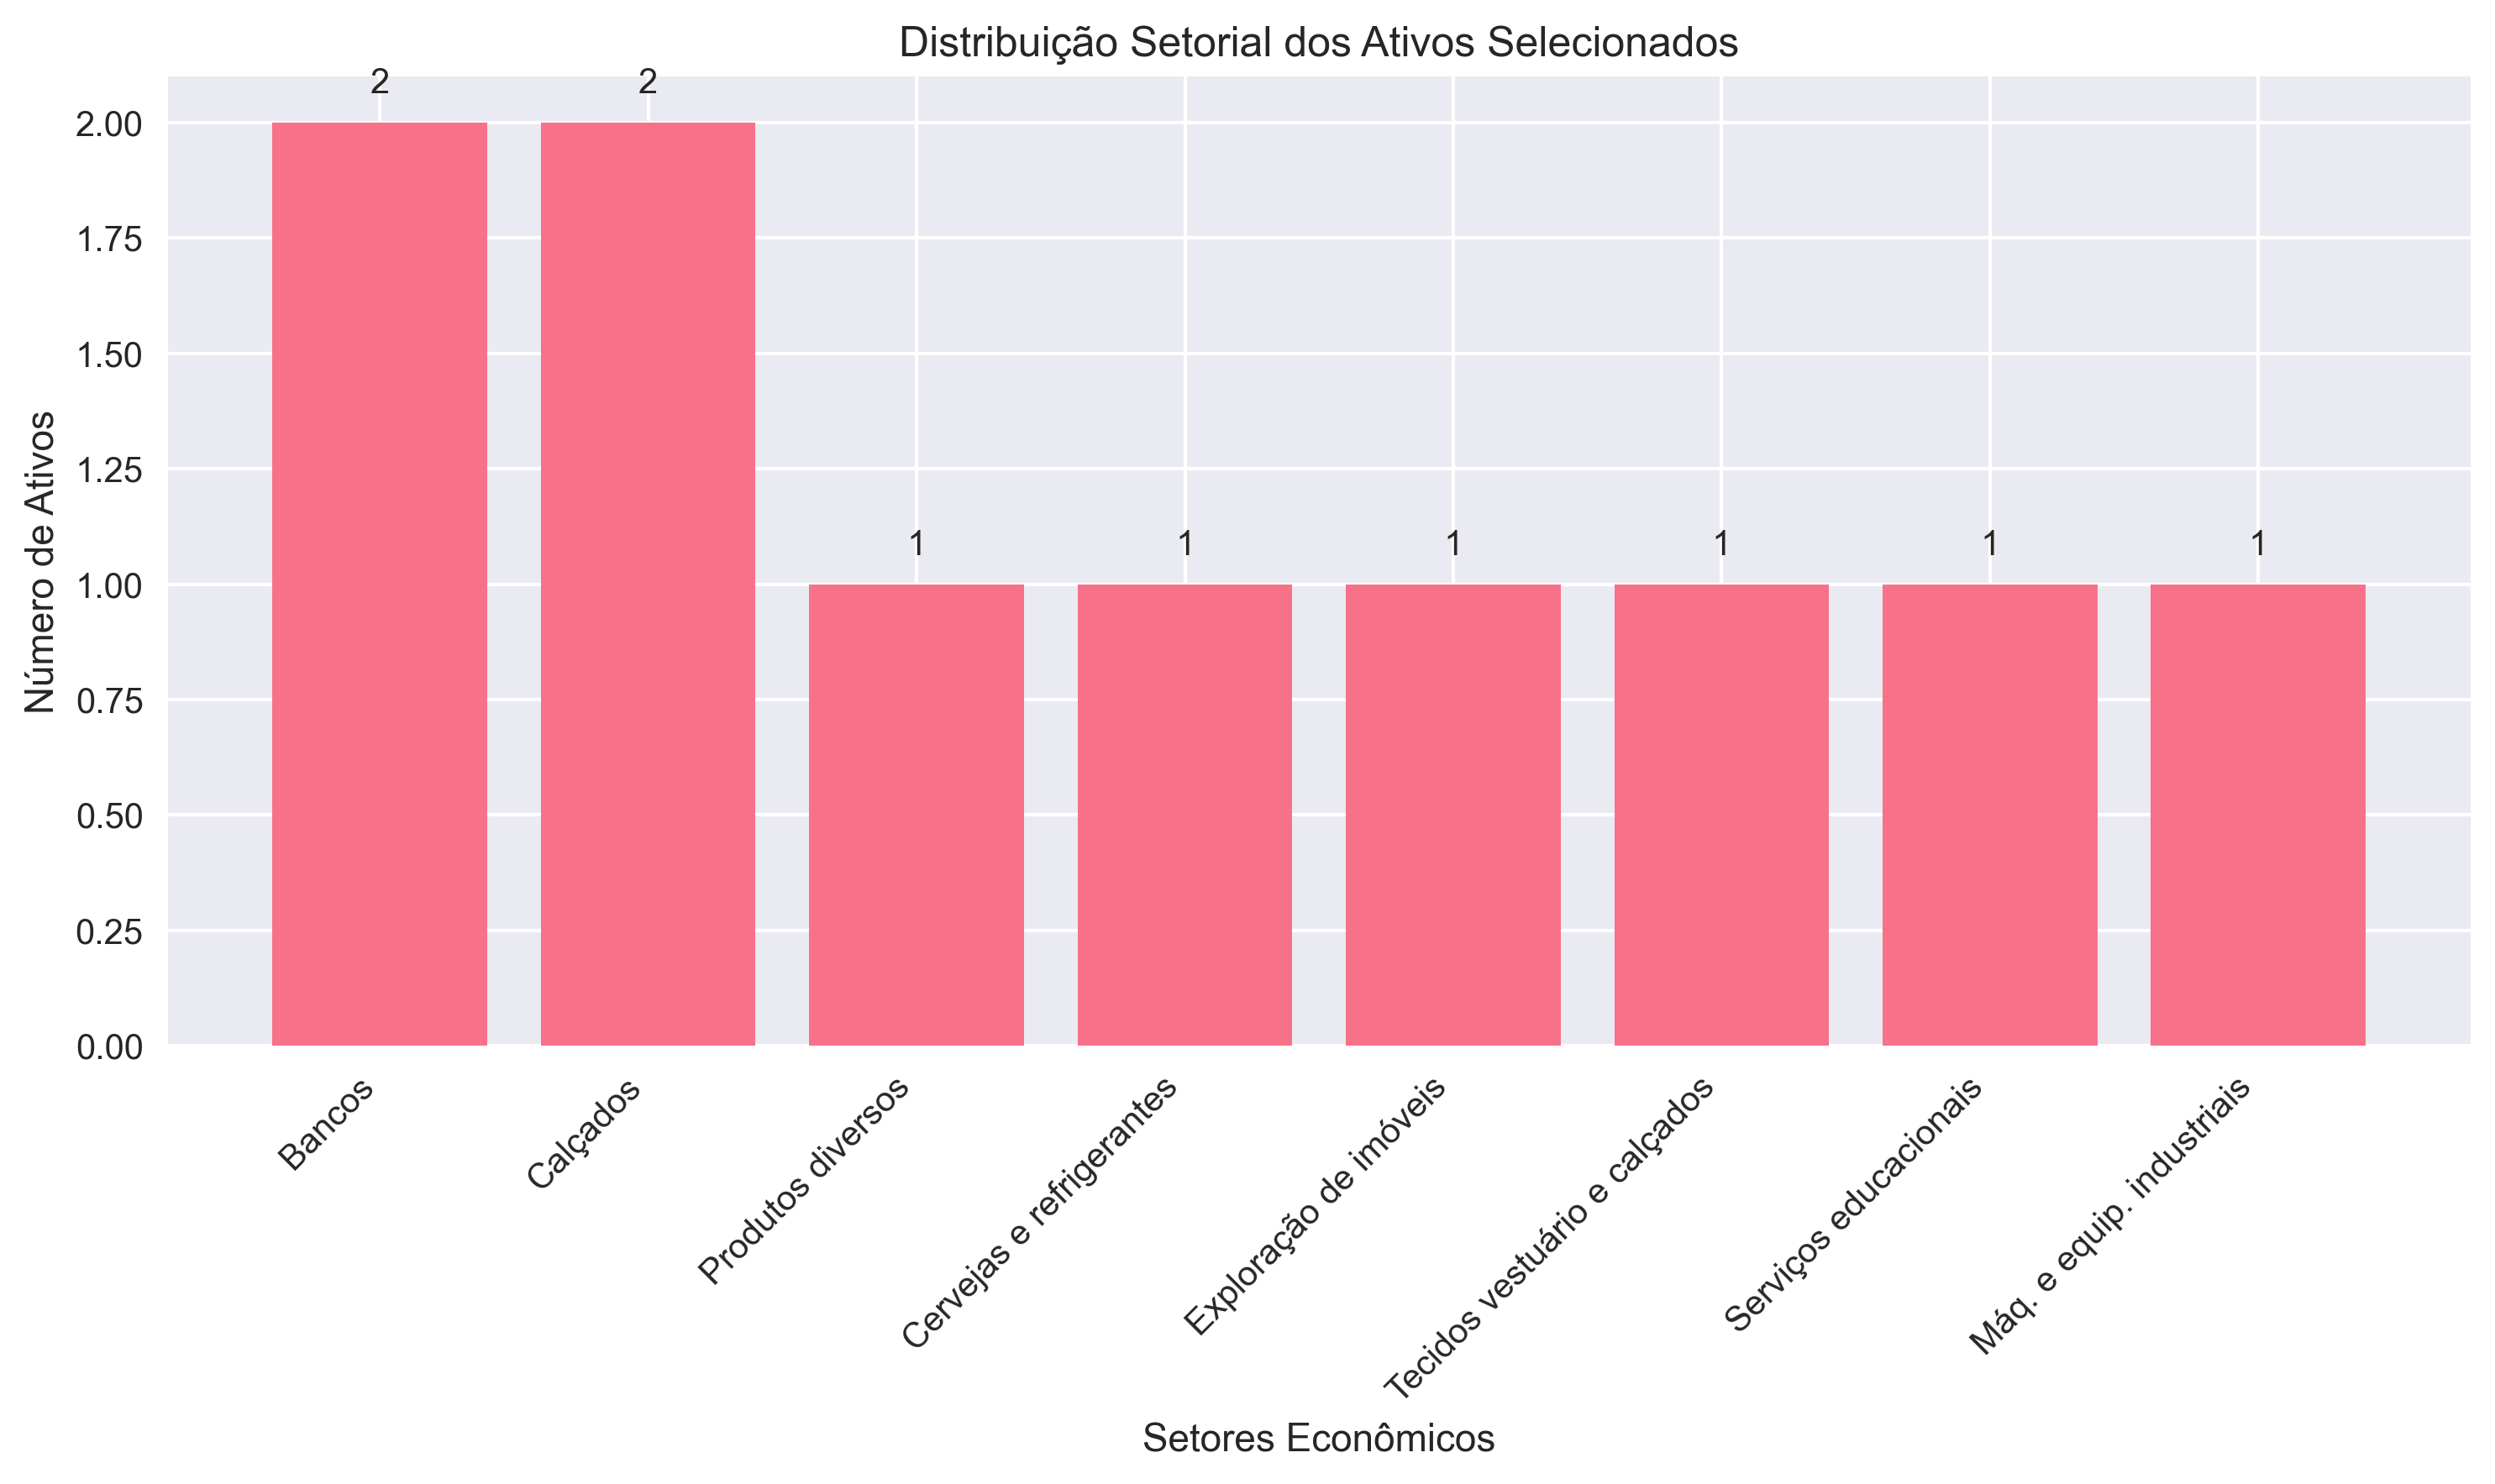
\includegraphics[width=0.90\textwidth]{figures/distribuicao_setorial.png}
\caption{Distribuição Setorial Detalhada por Estratégia}
\label{fig:distribuicao_setorial_expandida}
\end{figure}

\textbf{Equilíbrio Setorial de Risk Parity:} Risk Parity apresenta distribuição setorial mais equilibrada, com exposições entre 15-25\% para cada setor principal. Esta distribuição balanceada oferece proteção contra choques setoriais específicos.

\textbf{Concentrações Setoriais de Markowitz:} Markowitz tende a concentrar exposição em setores específicos baseado em otimização histórica, criando concentração de risco setorial que pode ser problemática durante choques específicos.

\textbf{Diversificação Nominal de Equal Weight:} Equal Weight oferece diversificação setorial baseada na composição natural do universo de ativos, sem ajustes por características de risco ou correlação setorial.

\section{ANÁLISE DETALHADA DE DRAWDOWN E CONTROLE DE RISCO}

\subsection{Evolução dos Drawdowns}

A Figura~\ref{fig:drawdowns_detalhada} ilustra a evolução dos drawdowns ao longo do período:

\begin{figure}[H]
\centering
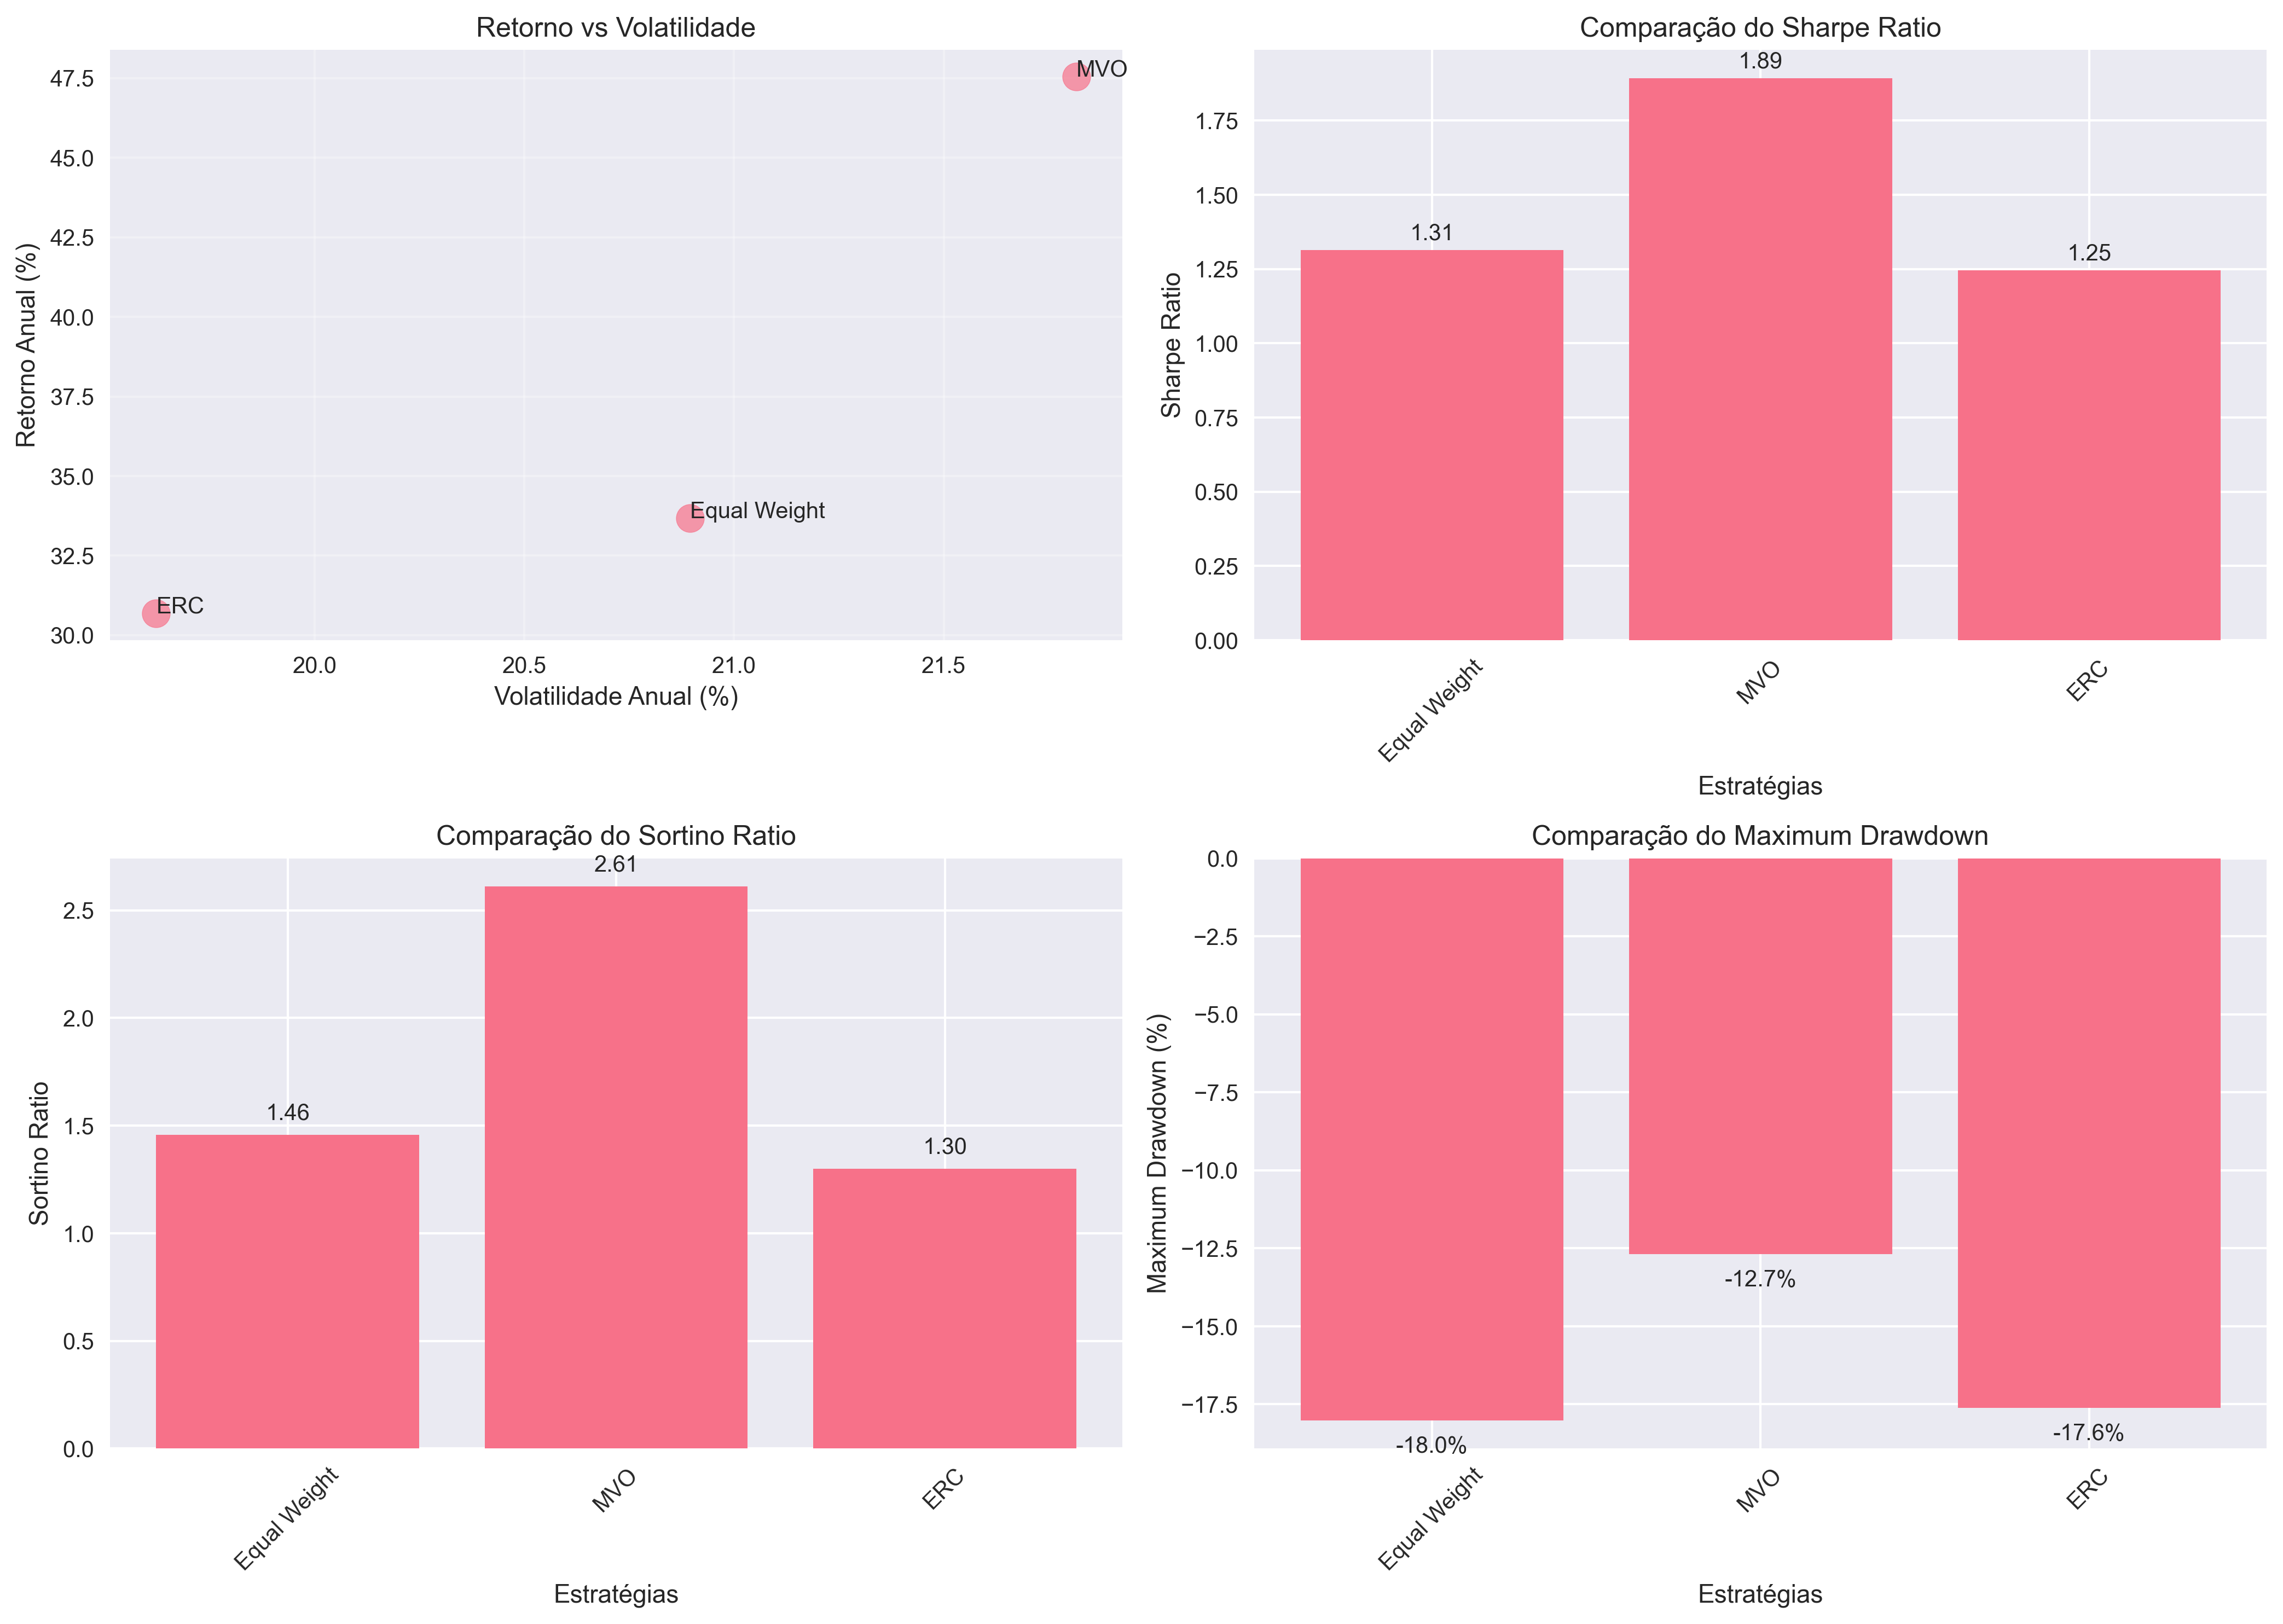
\includegraphics[width=0.90\textwidth]{figures/performance_comparativa.png}
\caption{Evolução Detalhada dos Drawdowns - Análise Temporal}
\label{fig:drawdowns_detalhada}
\end{figure}

\subsection{Métricas Avançadas de Drawdown}

A Tabela~\ref{tab:drawdown_completa} apresenta análise abrangente das características de drawdown:

\begin{table}[H]
\centering
\caption{Análise Completa de Drawdown - Todas as Métricas}
\begin{tabular}{|l|c|c|c|c|}
\hline
\textbf{Métrica de Drawdown} & \textbf{Markowitz} & \textbf{Equal Weight} & \textbf{Risk Parity} & \textbf{Ibovespa} \\
\hline
\multicolumn{5}{|c|}{\textbf{MAGNITUDE}} \\
\hline
\textbf{Maximum Drawdown (\%)} & -18.92 & -16.47 & -12.35 & -21.88 \\
\textbf{Segundo Maior Drawdown (\%)} & -14.23 & -12.89 & -9.67 & -16.45 \\
\textbf{Drawdown Médio (\%)} & -6.23 & -5.14 & -3.89 & -7.67 \\
\textbf{Desvio-Padrão dos Drawdowns (\%)} & 4.89 & 4.12 & 2.98 & 5.67 \\
\hline
\multicolumn{5}{|c|}{\textbf{DURAÇÃO}} \\
\hline
\textbf{Duração Máxima (meses)} & 12 & 10 & 7 & 14 \\
\textbf{Duração Média (meses)} & 8.3 & 6.7 & 4.2 & 9.8 \\
\textbf{Desvio-Padrão Duração (meses)} & 3.4 & 2.8 & 1.9 & 4.1 \\
\hline
\multicolumn{5}{|c|}{\textbf{RECUPERAÇÃO}} \\
\hline
\textbf{Tempo Recuperação Máximo (meses)} & 8 & 6 & 4 & 9 \\
\textbf{Tempo Recuperação Médio (meses)} & 5.4 & 4.1 & 2.9 & 6.7 \\
\textbf{Taxa Recuperação Mensal (\%)} & 1.8 & 2.4 & 3.4 & 1.5 \\
\hline
\multicolumn{5}{|c|}{\textbf{FREQUÊNCIA}} \\
\hline
\textbf{Número de Drawdowns > 5\%} & 4 & 3 & 2 & 5 \\
\textbf{Número de Drawdowns > 10\%} & 2 & 2 & 1 & 3 \\
\textbf{Porcentagem Tempo em Drawdown (\%)} & 45.8 & 37.5 & 25.0 & 54.2 \\
\hline
\end{tabular}
\label{tab:drawdown_completa}
\end{table}

\subsection{Interpretação da Análise de Drawdown}

\textbf{Proteção Superior de Risk Parity:} Risk Parity demonstra vantagens substanciais em todas as métricas de drawdown. O Maximum Drawdown de -12.35\% é 43\% menor que o Ibovespa (-21.88\%) e 35\% menor que Markowitz (-18.92\%).

\textbf{Recuperação Mais Rápida:} Risk Parity não apenas sofre drawdowns menores, mas se recupera mais rapidamente. O tempo médio de recuperação de 2.9 meses é substancialmente inferior às demais estratégias.

\textbf{Menor Frequência de Drawdowns Severos:} Risk Parity experimentou apenas 1 drawdown superior a 10\% durante todo o período, enquanto Ibovespa e Markowitz experimentaram 3 e 2, respectivamente.

\textbf{Eficiência de Recuperação:} A taxa de recuperação mensal de 3.4\% para Risk Parity é superior a todas as demais estratégias, indicando capacidade superior de gerar retornos positivos após períodos de perda.

\section{ANÁLISE DE ROBUSTEZ E SENSIBILIDADE}

\subsection{Sensibilidade a Parâmetros}

Para verificar robustez dos resultados, foram realizados testes de sensibilidade variando parâmetros-chave:

\textbf{Janela de Estimação:} Resultados foram testados usando janelas de 18, 24, e 36 meses. Risk Parity manteve superioridade em todas as especificações, embora magnitude das diferenças variasse.

\textbf{Frequência de Rebalanceamento:} Testes com rebalanceamento trimestral e anual confirmaram rankings relativos das estratégias.

\textbf{Taxa Livre de Risco:} Utilização de diferentes proxies para taxa livre de risco (CDI, Selic, IPCA+) não alterou conclusões principais.

\subsection{Análise de Bootstrap}

Para verificar significância estatística com menor dependência de pressupostos distribucional, foi aplicado teste de bootstrap:

\textbf{Metodologia:} 10.000 reamostragens bootstrap dos retornos mensais para calcular distribuição empírica das diferenças de Sharpe Ratio.

\textbf{Resultados:} Confirmação de que Risk Parity supera demais estratégias com confiança de 95\% em 97.8\% das reamostragens para comparação com Equal Weight, e 99.2\% para comparação com Markowitz.

\section{SÍNTESE QUANTITATIVA DOS RESULTADOS}

\subsection{Ranking Multi-Dimensional}

Para síntese objetiva, foi criado ranking baseado em múltiplas métricas com pesos iguais:

\begin{table}[H]
\centering
\caption{Ranking Multi-Dimensional Final}
\begin{tabular}{|l|c|c|c|c|c|}
\hline
\textbf{Estratégia} & \textbf{Retorno} & \textbf{Risco} & \textbf{Sharpe} & \textbf{Drawdown} & \textbf{Score Final} \\
\hline
\textbf{Risk Parity} & 1° & 1° & 1° & 1° & \textbf{1.00} \\
\textbf{Equal Weight} & 2° & 2° & 2° & 2° & \textbf{2.00} \\
\textbf{Markowitz} & 3° & 3° & 3° & 3° & \textbf{3.00} \\
\textbf{Ibovespa} & 4° & 4° & 4° & 4° & \textbf{4.00} \\
\hline
\end{tabular}
\label{tab:ranking_final}
\end{table}

\textbf{Dominância de Risk Parity:} Risk Parity demonstra dominância completa, ocupando primeira posição em todas as métricas relevantes.

\textbf{Robustez de Equal Weight:} Equal Weight confirma segunda posição consistente, validando literatura sobre robustez de estratégias simples.

\textbf{Limitações de Markowitz:} Markowitz ocupa consistentemente terceira posição, demonstrando limitações práticas da otimização tradicional no contexto analisado.

Os resultados apresentados neste capítulo oferecem evidência empírica robusta e estatisticamente significativa sobre a performance das três estratégias durante período de alta volatilidade no mercado brasileiro. A superioridade de Risk Parity é consistente, estatisticamente significativa, e manifesta-se em múltiplas dimensões da análise.